% EVALUATION
% ==========
%
% Results and their critical analysis should be reported, whether the
% results conform to expectations or otherwise and how they compare
% with other related work. Where appropriate evaluation of the work
% against the original objectives should be presented.

A total of \input{gen/num_scenarios} scenarios were tested. For each
scenario, an average of \input{gen/num_avg_params} unique workgroup
sizes were tested (max \input{gen/num_max_params}), for a total of
\input{gen/num_runtime_stats} combinations of scenario and workgroup
size. Runtimes were collected by randomly sampling $W_{safe}$, for an
average of \input{gen/avg_sample_count} runtimes per scenario (total
\input{gen/num_samples}). Figure~\ref{fig:min-max-runtimes} shows the
distribution of minimum and maximum runtimes.

\begin{figure}
\centering
\includegraphics{gen/img/min_max_runtimes}
\caption{%
  Distribution of minimum and maximum observed runtimes for each
  combination of scenario and parameter value, normalised to their
  respective mean runtimes.%
}
\label{fig:min-max-runtimes}
\end{figure}

The relative performance of different workgroup sizes for a scenario
can be found by normalising the mean runtimes against that of the
oracle workgroup size. This can provide an upper limit on the speedup
which can be attained using autotuning as the reciprocal of the
normalised runtime for the workgroup size which gave the lowest
performance. Applying this to all scenarios, we find the upper limit
of potential speedup to be between
$\input{gen/min_possible_speedup}\times$ --
$\input{gen/max_possible_speedup}\times$ (average
$\input{gen/avg_possible_speedup}\times$). This demonstrates that
selection of the optimal

Figure~\ref{fig:max-wgsizes} shows the distribution of maximum
workgroup sizes across all scenarios. Figure~\ref{fig:oracle-wgsizes}
shows the distribution of oracle workgroup sizes. Clearly, the
workgroup size $64 \times 4$ is the optimal value across the most
scenarios, but even that proves optimal only 10\% of the time. As
Figure~\ref{fig:oracle-accuracy} shows,
\input{gen/num_wgsizes_50_accuracy} unique workgroup sizes are
required in order to achieve oracle performance just 50\% of the time.


\begin{figure}
\begin{subfigure}[t]{0.32\textwidth}
\centering
\includegraphics{gen/img/performance_kernels.png}
\vspace{-1.5em} % Shrink vertical padding
\caption{Kernels}
\label{fig:performance-kernels}
\end{subfigure}
~%
\begin{subfigure}[t]{0.32\textwidth}
\centering
\includegraphics{gen/img/performance_devices.png}
\vspace{-1.5em} % Shrink vertical padding
\caption{Devices}
\label{fig:performance-devices}
\end{subfigure}
~%
\begin{subfigure}[t]{0.32\textwidth}
\centering
\includegraphics{gen/img/performance_datasets.png}
\vspace{-1.5em} % Shrink vertical padding
\caption{Datasets}
\label{fig:performance-datasets}
\end{subfigure}
\label{fig:performance}
\caption{%
  Relative performance of workgroup sizes for different
  scenarios, divided by kernels, devices, and datasets.%
}
\end{figure}


\begin{figure}
\begin{subfigure}[t]{0.45\textwidth}
\centering
\includegraphics{gen/img/max_wgsizes.png}
\vspace{-1.5em} % Shrink vertical padding
\caption{Maximum workgroup sizes}
\label{fig:max-wgsizes}
\end{subfigure}
~%
\begin{subfigure}[t]{0.45\textwidth}
\centering
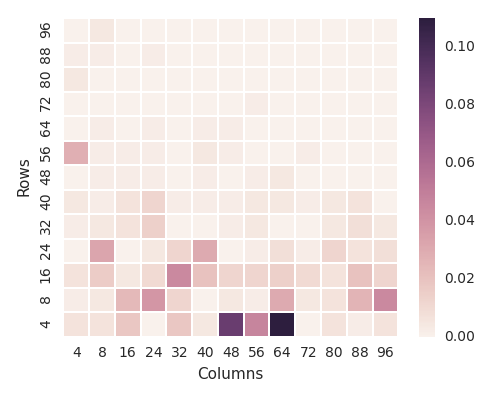
\includegraphics{gen/img/oracle_param_space.png}
\vspace{-1.5em} % Shrink vertical padding
\caption{Oracle workgroup sizes}
\label{fig:oracle-wgsizes}
\end{subfigure}
\caption{%
  On the left, the distribution of maximum legal workgroup sizes for
  all scenarios. On the right, the distribution of oracle workgroup
  sizes.%
}
\label{fig:heatmaps}
\end{figure}


\begin{figure}
\centering
\includegraphics{gen/img/num_params_oracle.png}
\caption{%
  Accuracy compared to the oracle as a function of the number of
  workgroup sizes used. The best accuracy that is achievable using a
  single statically chosen value is
  \protect\input{gen/max_oracle_param_frequency}\%.%
}
\label{fig:oracle-accuracy}
\end{figure}

\begin{figure}
\centering
\includegraphics{gen/img/params_summary.png}
\caption{%
  The red line shows the ``legality'' of the parameter value, i.e.\
  the ratio of scenarios for which that workgroup size is legal.  The
  blue and green lines show the geometric mean of the performance of
  workgroup sizes relative to the oracle for: all scenarios, and only
  the scenarios for which the workgroup size is legal.%
}
\end{figure}

\begin{figure}
\centering
\includegraphics{gen/img/performance_max_wgsize.png}
\caption{%
  Performance of a workgroup size relative to the oracle vs the
  maximum legal workgroup size. There is no clear trend between the
  performance of a workgroup size and it's size relative to the
  maximum allowed.%
}
\end{figure}


\TODO{Evaluate the effectiveness of training with synthetic
  benchmarks.}

% P. J. Fleming and J. J. Wallace, “How not to lie with statistics:
% the correct way to summarize benchmark results,” Commun. ACM,
% vol. 29, no. 3, pp. 218–221, 1986.
\TODO{%
  How to properly report benchmark results~\cite{Fleming1986}.%
}

% A. Georges, D. Buytaert, and L. Eeckhout, “Statistically Rigorous
% Java Performance Evaluation,” in Proceedings of the 22Nd Annual ACM
% SIGPLAN Conference on Object-oriented Programming Systems and
% Applications, 2007, vol. 42, no. 10, p. 57.
\TODO{%
  Statistically rigorous performance evaluations.~\cite{Georges2007}.
}
